In this section the experimental results are presented. The following algorithms are used to solve the 6 categories of games:
\begin{enumerate}
	\item Zielonka's recursive algorithm, product based
	\item Fixed-point iteration, product based
	\item Fixed-point iteration, local product based
	\item Zielonka's recursive algorithm, family based with explicit configuration representation
	\item Zielonka's recursive algorithm, family based with symbolic configuration representation
	\item Incremental pre-solve algorithm
	\item Incremental pre-solve algorithm, local
\end{enumerate}

The numbers presented are the times it took to solve the games; times for parsing, projecting (for product based approaches) and printing solutions are excluded. So the product based results are the sum of the solve times of the projections, parsing and projecting are not included in the result.

The exact times can be found in appendix \ref{appendix:resultsexact}, in this section the results are visualized and presented to be easily interpreted. In some cases the results in a graph are normalized meaning that the running times are divided by the running times of the first algorithm in the graph. Specifically for the random games the running times vary a lot so normalizing is required to properly visualize the results. The times are presented on a logarithmic scale, games that were unable to be completed (due to memory) are marked with a grey bar.

All the experiments are ran on a Linux x64 operating system with an Intel i5-4570 processor and 8GB of DDR3 RAM.
\subsection{Zielonka's family based}
First we compare the running times of the Zielonka's family based approaches with the Zielonka's product based approach. First we look at the model verification games.
\begin{figure}[H]
	\includegraphics[width=1\linewidth]{"results/minepump/Zlnk product based_Zlnk fam based - explicit_Zlnk fam based - symbolic_.svg"}
	\caption{Running time of Zielonka's algorithms on the minepump problem}
	\label{fig:minepumpzlnks}
\end{figure}%
\begin{figure}[H]
	\includegraphics[width=1\linewidth]{"results/elevator/Zlnk product based_Zlnk fam based - explicit_Zlnk fam based - symbolic_.svg"}
	\caption{Running time of Zielonka's algorithms on the elevator problem}
	\label{fig:elevatorzlnks}
\end{figure}%
We can see that the performance of the explicit variant varies a lot between games. The symbolic variant greatly outperforms the product based approach for every problem.

Next we inspect the random games, first we look at the games with a variable $\lambda$ and a random number of features. The graphs are normalized.
\begin{figure}[H]
\includegraphics[width=1\linewidth]{"results/FF_randomgames/Zlnk product based_Zlnk fam based - explicit_Zlnk fam based - symbolic_.svg"}
\caption{Running time of Zielonka's algorithms on randomgames of type 1 with $\lambda = \frac{\textit{game nr}}{100}$, times are normalized}
\label{fig:elevatorzlnks}
\end{figure}%
\begin{figure}[H]
\includegraphics[width=1\linewidth]{"results/FC_randomgames/Zlnk product based_Zlnk fam based - explicit_Zlnk fam based - symbolic_.svg"}
\caption{Running time of Zielonka's algorithms on randomgames of type 2 with $\lambda = \frac{\textit{game nr}}{100}$, times are normalized}
\label{fig:elevatorzlnks}
\end{figure}%
\begin{figure}[H]
\includegraphics[width=1\linewidth]{"results/BC_randomgames/Zlnk product based_Zlnk fam based - explicit_Zlnk fam based - symbolic_.svg"}
\caption{Running time of Zielonka's algorithms on randomgames of type 3 with $\lambda = \frac{\textit{game nr}}{100}$, times are normalized}
\label{fig:elevatorzlnks}
\end{figure}%
For type 1 games we see that when $\lambda$ gets bigger the family based symbolic approach starts winning from the product based approach. There are a few exceptions to this, games 80, 82 and 86, all three of these games have only 4 features. As we will see later the less features there are in a game the worse the family based approaches perform.

For type 2 the explicit variant performs very similar to the type 1 games, however the symbolic approach performs much worse. This is due to the unstructured nature of the configuration sets which negatively influences bdd performance but has no effect on the explicit set operations. We also see the explicit algorithm outperforming the symbolic algorithm in some cases.

For type 3 games the product based approach performs generally better than the family based approaches unless $\lambda$ becomes very high.

Next we inspect how the algorithms scales in terms of number of features
\begin{figure}[H]
\includegraphics[width=1\linewidth]{"results/randomscalegames/Zlnk product based_Zlnk fam based - explicit_Zlnk fam based - symbolic_.svg"}
\caption{Running time of Zielonka's algorithms on randomgames of type 1 with $\lambda = 0.92$ and the number of features equal to the $\textit{game nr}$, times are normalized}
\label{fig:elevatorzlnks}
\end{figure}%
We can clearly conclude that as the number of features increases the family based symbolic approach performs better compared to the product based approach.

Overall we can conclude that the explicit algorithm performs somewhat arbitrary, however the symbolic algorithm performs really well for model checking problems and random games that have similar properties. Also we can conclude that the algorithms scales well in terms of number of features.


\subsection{Incremental pre-solve algorithm}
We compare the running times of the incremental pre-solve approaches with the fixed-point iteration product based algorithm. First we look at the model verification games.
\begin{figure}[H]
	\includegraphics[width=1\linewidth]{"results/minepump/Fixed-point product based_Incremental pre-solve_.svg"}
	\caption{Running time of the incremental pre-solve algorithms on the minepump problem}
	\label{fig:minepumpzlnks}
\end{figure}%
\begin{figure}[H]
	\includegraphics[width=1\linewidth]{"results/elevator/Fixed-point product based_Incremental pre-solve_.svg"}
	\caption{Running time of the incremental pre-solve algorithms on the elevator problem. Game 3, 4 and 5 were not able to be finished }
	\label{fig:elevatorzlnks}
\end{figure}%
The incremental pre-solve algorithms does not show any significant improvements over the product based fixed-point algorithm.

Next we inspect the random games, first we look at the games with a variable $\lambda$ and a random number of features. The graphs are normalized.
\begin{figure}[H]
	\includegraphics[width=1\linewidth]{"results/FF_randomgames/Fixed-point product based_Incremental pre-solve_.svg"}
	\caption{Running time of the incremental pre-solve algorithms on randomgames of type 1 with $\lambda = \frac{\textit{game nr}}{100}$, times are normalized}
	\label{fig:type1FPIteglobal}
\end{figure}%
\begin{figure}[H]
	\includegraphics[width=1\linewidth]{"results/FC_randomgames/Fixed-point product based_Incremental pre-solve_.svg"}
	\caption{Running time of incremental pre-solve algorithms on randomgames of type 2 with $\lambda = \frac{\textit{game nr}}{100}$, times are normalized}
	\label{fig:elevatorzlnks}
\end{figure}%
\begin{figure}[H]
	\includegraphics[width=1\linewidth]{"results/BC_randomgames/Fixed-point product based_Incremental pre-solve_.svg"}
	\caption{Running time of incremental pre-solve algorithms on randomgames of type 3 with $\lambda = \frac{\textit{game nr}}{100}$, times are normalized}
	\label{fig:elevatorzlnks}
\end{figure}%
For type 1 and type 2 games we see that when $\lambda$ gets bigger the incremental pre-solve start performing better, however it this trends only appears when $\lambda$ get larger than about $0.95$.

Again we see that for type 3 games the family based algorithm performs worse.

Next we inspect how the algorithms scales in terms of number of features
\begin{figure}[H]
	\includegraphics[width=1\linewidth]{"results/randomscalegames/Fixed-point product based_Incremental pre-solve_.svg"}
	\caption{Running time of incremental pre-solve algorithms on randomgames of type 1 with $\lambda = 0.92$ and the number of features equal to the $\textit{game nr}$, times are normalized}
	\label{fig:elevatorzlnks}
\end{figure}%
There is a downwards trend when it comes to the number of features, however it is quite inconsistent. Note that these games have $\lambda=0.92$. Which is lower than the threshold observed in Figure \ref{fig:type1FPIteglobal}.

Overall the performance is not a significant improvement on the product based approach.
\subsection{Incremental pre-solve local algorithm}
Next we again compare the incremental pre-solver with the fixed-point iteration product based approach, however this time we compare the local variants. We start with the model-checking games.
\begin{figure}[H]
	\includegraphics[width=1\linewidth]{"results/minepump/Fixed-point local product based_Incremental pre-solve local_.svg"}
	\caption{Running time of the incremental pre-solve local algorithms on the minepump problem}
	\label{fig:minepumpzlnks}
\end{figure}%
\begin{figure}[H]
	\includegraphics[width=1\linewidth]{"results/elevator/Fixed-point local product based_Incremental pre-solve local_.svg"}
	\caption{Running time of the incremental pre-solve local algorithms on the elevator problem}
	\label{fig:elevatorzlnks}
\end{figure}%
Generally the performance of the incremental pre-solver local algorithm is better, also games 3, 4 and 5 for the elevator problem were solved which was not the case for the global algorithm.

Next we inspect the random games, first we look at the games with a variable $\lambda$ and a random number of features. The graphs are normalized.
\begin{figure}[H]
	\includegraphics[width=1\linewidth]{"results/FF_randomgames/Fixed-point local product based_Incremental pre-solve local_.svg"}
	\caption{Running time of the incremental pre-solve local algorithms on randomgames of type 1 with $\lambda = \frac{\textit{game nr}}{100}$, times are normalized}
	\label{fig:elevatorzlnks}
\end{figure}%
\begin{figure}[H]
	\includegraphics[width=1\linewidth]{"results/FC_randomgames/Fixed-point local product based_Incremental pre-solve local_.svg"}
	\caption{Running time of incremental pre-solve local algorithms on randomgames of type 2 with $\lambda = \frac{\textit{game nr}}{100}$, times are normalized}
	\label{fig:elevatorzlnks}
\end{figure}%
\begin{figure}[H]
	\includegraphics[width=1\linewidth]{"results/BC_randomgames/Fixed-point local product based_Incremental pre-solve local_.svg"}
	\caption{Running time of incremental pre-solve local algorithms on randomgames of type 3 with $\lambda = \frac{\textit{game nr}}{100}$, times are normalized}
	\label{fig:elevatorzlnks}
\end{figure}%
For type 1 games the local incremental pre-solve algorithm greatly outperforms the product based approach, for type 2 games this is still the case but we can see differences becoming a bit smaller. Finally for type 3 games it only outperforms the product based approach when $\lambda$ gets sufficiently high.

Next we inspect how the algorithms scales in terms of number of features
\begin{figure}[H]
	\includegraphics[width=1\linewidth]{"results/randomscalegames/Fixed-point local product based_Incremental pre-solve local_.svg"}
	\caption{Running time of incremental pre-solve local algorithms on randomgames of type 1 with $\lambda = 0.92$ and the number of features equal to the $\textit{game nr}$, times are normalized}
	\label{fig:elevatorzlnks}
\end{figure}%
Clearly the performance improves when the number of features becomes larger.

We can conclude that for model-checking games the algorithm performs decent, however the biggest improvements are seen on random games.
\subsection{Comparison}
After comparing family based and product based variants of the same algorithm we compare the algorithms overall. We do so by comparing the mean solve time of every set of games.

First we compare the independent algorithms. Table \ref{tab_compare_independent_algs} shows for every set of VPGs how long on average it took each algorithm to solve a VPG in that set.
\begin{table}[h]
	\centering
	\begin{tabular}{|l|l|l|l|l|}
		\hline
		& Zlnk & & Fixed-point & \\
		& & local & & local \\
		\hline
		minepump& 113 ms& 97 ms& 4606 ms& 4474 ms\\ \hline
		elevator& 35062 ms& 28399 ms& 9733571 ms& 1707949 ms\\ \hline
		FF randomgames& 314 ms& 288 ms& 64119 ms& 47106 ms\\ \hline
		FC randomgames& 312 ms& 288 ms& 53218 ms& 39947 ms\\ \hline
		BC randomgames& 318 ms& 307 ms& 44561 ms& 36483 ms\\ \hline
		randomscalegames& 756 ms& 697 ms& 75579 ms& 43983 ms\\ \hline
	\end{tabular}
	\caption{Comparison of independent algorithms}
	\label{tab_compare_independent_algs}
\end{table}

In table \ref{tab_compare_collective_algs} we compare the performance of the collective algorithms.
\begin{table}[h]
	\centering
	\begin{tabular}{|l|l|l|l|l|l|l|}
		\hline
		& Zlnk& & & & Incremental& \\
		& explicit & & symbolic & & pre-solve &
		\\
		&  & local & & local & & local
		\\ \hline
		minepump& 112 ms& 103 ms& 16 ms& 15 ms& 1153 ms& 671 ms\\ \hline
		elevator& 105856 ms& 36380 ms& 6674 ms& 5337 ms& 1065377 ms& 378460 ms\\ \hline
		FF randomgames& 324 ms& 329 ms& 3489 ms& 3488 ms& 28900 ms& 22716 ms\\ \hline
		FC randomgames& 506 ms& 514 ms& 50286 ms& 47707 ms& 118559 ms& 108023 ms\\ \hline
		BC randomgames& 540 ms& 535 ms& 38619 ms& 37885 ms& 145491 ms& 128929 ms\\ \hline
		randomscalegames& 28 ms& 24 ms& 2 ms& 2 ms& 1727 ms& 594 ms\\ \hline
	\end{tabular}
	\caption{Comparison of collective algorithms}
	\label{tab_compare_collective_algs}
\end{table}